Upplýsingar eru sjaldnast geymdar í gagnagrunnum upplýsinganna vegna. Markmiðið með að geyma upplýsingar er að gera það mögulegt að ná í þær aftur seinna.

Til að ná í upplýsingar notum við svokallaða \verb|SELECT| skipun. Þetta er skipun sem við munum koma til með að nota mikið og kynnast vel.

Hver \verb|SELECT| skipun er \emph{lýsing} á einhverjum upplýsingum sem við viljum fá. Við lýsum því hvaða upplýsingar við viljum, gagnagrunnskerfið sér svo um að finna þær fyrir okkur.
\section{SELECT}
Allar \verb|SELECT| skipanir innihalda að minnsta kosti lýsingu á því hvaða upplýsingar þarf að ná í.

Dæmi um ofurlitla \verb|SELECT| skipun má sjá í sýnidæmi \ref{sql:k4d1-summa}.

\begin{example}
\caption[Lágmarks SELECT]{Lítil \emph{SELECT} skipun. Hún inniheldur lýsingu á því hvaða upplýsingar á að finna: summuna $2+2$. Gagnagrunnskerfið getur reiknað hana út fyrir okkur.}
\label{sql:k4d1-summa}
\centering
\sql{sql/k4d1-summa.sql}
\end{example}

\subsection{SELECT - FROM}
\label{undirkafli:from}
Þegar \verb|SELECT| skipun er skrifuð er það oftast í þeim tilgangi að ná upplýsingum úr SQL-töflu.

Þegar ná á upplýsingum úr töflu þarf að minnsta kosti tvennt að koma fram - hvar upplýsingarnar er að finna og hvaða upplýsingar skal velja. Þetta má gera í eftirfarandi skrefum:
\newpage
\begin{enumerate}
 \item Skrifa orðið \verb|SELECT| (sem gerir skipunina að \verb|SELECT| skipun)
 \item Skrifa nöfn dálkanna sem velja skal
 \item Skrifa orðið \verb|FROM|
 \item Skrifa nafn töflunnar sem velja skal úr.
\end{enumerate}
Fyrri tvö skrefin lýsa þá því hvaða upplýsingar skal velja, þau seinni tvö lýsa því hvaðan þær koma.\footnote{Seinni tvö skrefin lýsa svokallaðri \emph{FROM} klausu. \emph{FROM} klausa lýsir því hvaðan upplýsingar koma. Oft er þetta bara nafn á einni töflu.}

\verb|SELECT| skipun með \verb|FROM| klausu má sjá á sýnidæmi \ref{sql:k4d2-from}.

\begin{table}
\centering
\caption[Nemendur]{Nokkrir uppskáldaðir nemendur fæddir árið 1998. Við munum velja upplýsingar úr þessari töflu í næstu sýnidæmum.}
\label{tafla:nemendur}
\begin{tabular}{llll}
\toprule
numer&nafn&kennitala&innritun\\
\midrule
1&Magnús Ásgeir Steinþórsson&090698-6489& 2014-07-01\\
2&Sigurður Ómarsson&251198-1369& 2014-06-04\\
3&Róbert Marinó Björnsson&060998-2489& 2014-07-14\\
4&Konráð Hreinn Aðalsteinsson&120498-8869& 2014-06-02\\
5&Jón Guðmundsson&230598-2159& 2014-07-03\\
6&Birgir Torfason&170798-7249& 2014-06-06\\
7&Höskuldur Frímann Ásmundsson&020298-4139& 2014-07-08\\
8&Jón Guðmundsson&210498-7889& 2014-06-11\\
9&Hilmar Hjartarson&020798-4599& 2014-07-16\\
10&Reynir Rafn Sigurgeirsson&211298-7239& 2014-06-12\\
11&Ingunn Rún Andradóttir&161298-1589& 2014-07-05\\
12&Pálína Björk Þórólfsdóttir&030798-0829& 2014-06-09\\
13&Regína Sigrún Jensdóttir&140798-6499& 2014-07-08\\
14&Líney Geirsdóttir&111098-3289& 2014-06-21\\
15&Steinunn Berglind Eiðsdóttir&190398-1889& 2014-07-04\\
16&Kristjana Ólafsdóttir&230298-4759& 2014-06-01\\
17&Þóra Gestsdóttir&010498-8489& 2014-07-05\\
18&Kolfinna Svava Óttarsdóttir&210498-5759& 2014-06-02\\
19&Elísabet Hrannarsdóttir&050298-3109& 2014-07-09\\
20&Hafrún Þorláksdóttir&250498-2849& 2014-06-19\\
\bottomrule
\end{tabular}
\end{table}

\begin{example}
\caption[SELECT FROM]{\emph{SELECT} skipun með \emph{FROM} klausu. Hún velur allan ``nafn'' dálkinn úr töflunni Nemendur (\ref{tafla:nemendur}).}
\label{sql:k4d2-from}
\centering
\sql{sql/k4d2-from.sql}
\end{example}

\begin{figure*}
\caption[Niðurstöður SELECT í Workbench]{Hér sést hvernig keyra má \emph{SELECT} skipunina úr sýnidæmi \ref{sql:k4d2-from} í MySQL Workbench. Skipunin er í aðalglugganum, niðurstaða hennar sést fyrir neðan.}
\label{mynd:workbench-select}
\centering
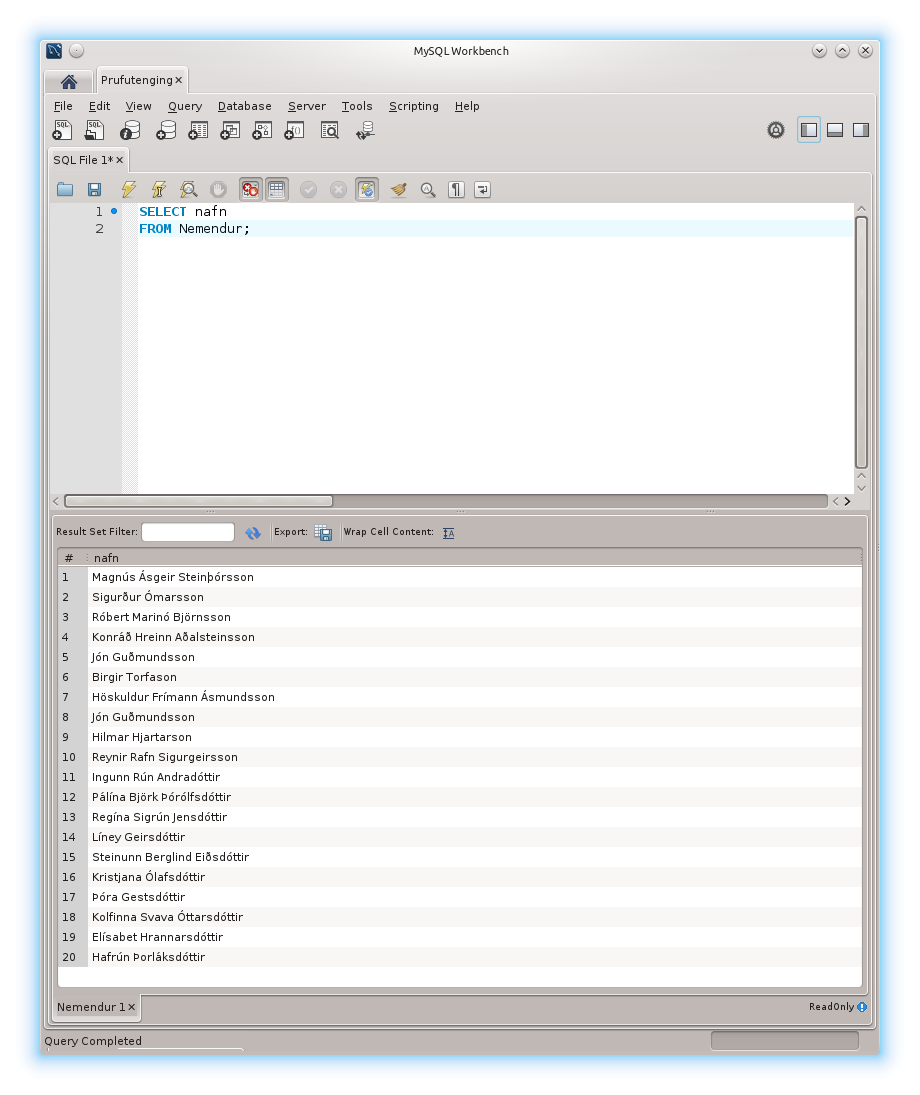
\includegraphics[width=\linewidth]{myndir/workbench-select}
\end{figure*}

\verb|SELECT| skipun getur náð í marga dálka (eða mörg atriði) í einu. Atriðin eru þá einfaldlega aðgreind með kommum. Þetta má sjá á mynd \ref{mynd:workbench-nidurstada-margir-dalkar}.

\begin{figure*}
\caption[Niðurstöður margra dálka SELECT í Workbench]{\emph{SELECT} skipun sem nær í marga dálka getur litið út á þessa leið í MySQL workbench. Allar upplýsingarnar úr dálkunum ``nafn'' og ``kennitala'' voru valdar. Aðrir dálkar sjást ekki.}
\label{mynd:workbench-nidurstada-margir-dalkar}
\centering
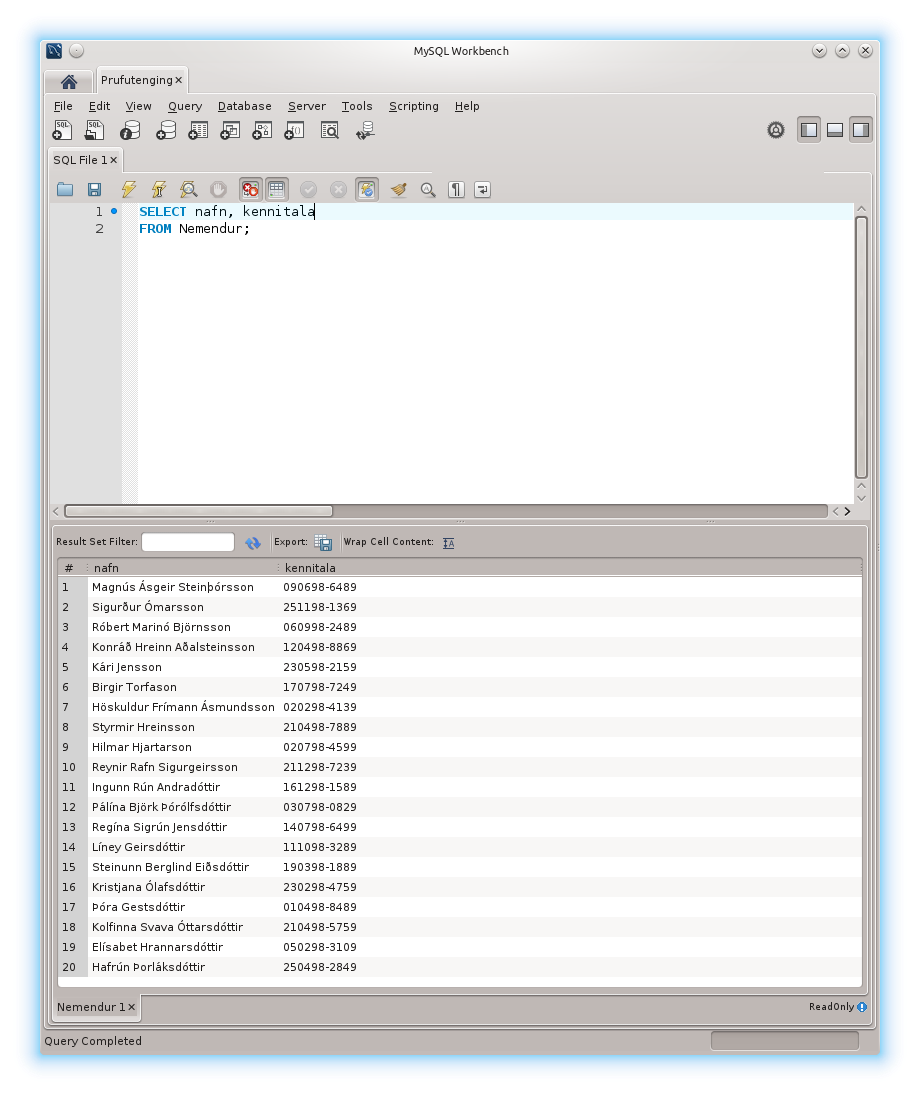
\includegraphics[width=\linewidth]{myndir/workbench-nidurstada-margir-dalkar}
\end{figure*}

\newpage
\section{WHERE klausan}
Hingað til höfum við valið heila dálka með \verb|SELECT| skipunum. Það sem við viljum hins vegar oftast gera er að finna ákveðnar upplýsingar í töflunni, frekar en að fá þær allar.

Til þess að fá bara þær upplýsingar sem við viljum búum við til ``síu''\footnote{e. \emph{filter}} sem hleypir engum upplýsingum í gegn nema þeim sem við viljum.

Slík sía þarf að innihalda lýsingu á þeim gögnum sem hún á að hleypa á í gegn. Það er gert í klausu sem við köllum \verb|WHERE| klausu og kemur fyrir aftan \verb|FROM| klausuna. Dæmi um þetta má sjá í sýnidæmum \ref{sql:k4d4-where-numer} til \ref{mynd:workbench-nidurstada-jon}.

\begin{example}
\caption[SELECT með WHERE klausu - eftir númeri][-1cm]{\emph{SELECT} skipun með \emph{WHERE} klausu sem nær í nafn nemanda (úr töflu \ref{tafla:nemendur}) þar sem ``numer'' dálkurinn er með gildið 11. Hún skilar einni línu, nafninu Ingunn Rún Andradóttir.}
\label{sql:k4d4-where-numer}
\centering
\sql{sql/k4d4-where-numer.sql}
\end{example}

\begin{example}
\caption[SELECT með WHERE klausu - eftir nafni]{\emph{SELECT} skipun með \emph{WHERE} klausu sem nær í kennitölu nemanda eftir nafni hans. Hún skilar einni línu, kennitölunni 251198-1369.}
\label{sql:k4d5-where-nafn}
\centering
\sql{sql/k4d5-where-nafn.sql}
\end{example}

\begin{example}
\caption[SELECT með WHERE klausu - endurtekin gildi]{Skilyrðið sem sett er fram í \emph{WHERE} klausu getur átt við meira en eina línu í töflunni. Þessi skipun finnur nöfn og kennitölu allra sem heita Jón Guðmundsson. Þeir reynast vera tveir, með kennitölurnar 230598-2159 og 210498-7889.}
\label{sql:k4d6-where-nafn-endurtekid}
\centering
\sql{sql/k4d6-where-nafn-endurtekid.sql}
\end{example}

\begin{figure*}[h]
\caption[Niðurstöður margra dálka SELECT í Workbench]{Hér sést sýnidæmi \ref{sql:k4d6-where-nafn-endurtekid} í MySQL Workbench.}
\label{mynd:workbench-nidurstada-jon}
\centering
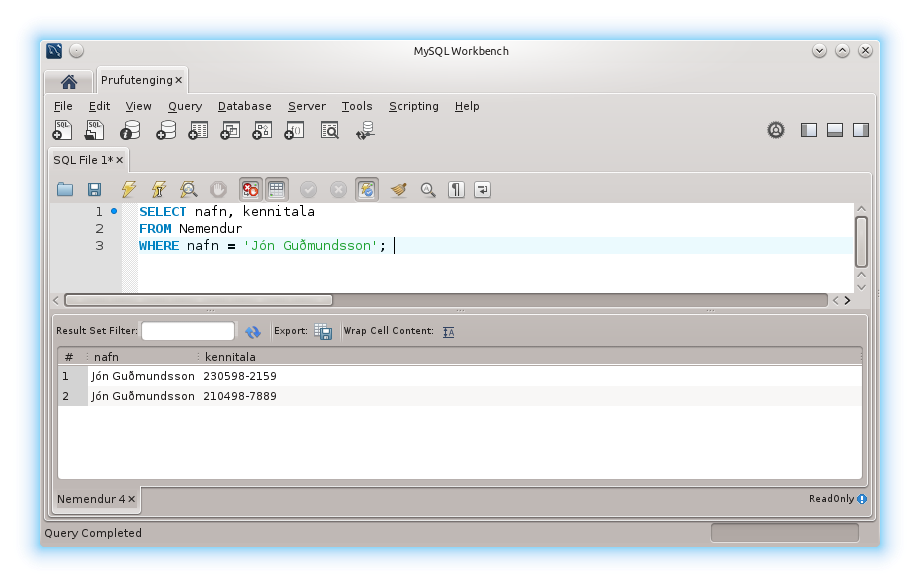
\includegraphics[width=\linewidth]{myndir/workbench-nidurstada-jon}
\end{figure*}
\subsection{Röksegðir}
\label{undirkafli:roksegdir}
Í öllum \verb|WHERE| klausunum hér á undan er um að ræða síur sem ekki hleypa neinum línum í gegn nema að þær uppfylli eitt, nákvæmt skilyrði. Skilyrðið í sýnidæmi \ref{sql:k4d4-where-numer}, \verb|numer = 11|, hleypir til dæmis einungis þeim nemanda sem er með nákvæmlega númerið 11 í gegn.

Skilyrðin geta þó verið margs konar. \verb|WHERE| klausan tekur nefnilega við næstum hvaða röksegð\footnote{e. \emph{boolean expression}} sem er, þ.e.a.s. alls kyns samanburðum og staðhæfingum sem að lokum gefa gildin ``satt'' eða ``ósatt''.\footnote{Í MySQL er ``satt'' táknað með tölunni $1$ eða orðinu \emph{TRUE}. ``Ósatt'' er táknað með $0$ eða \emph{FALSE}.}

\newpage
Orðið ``röksegð'' kann að hljóma undarlega, en um kunnuglegt fyrirbæri er að ræða. ``Skilyrðið'' \verb|numer = 11| er til dæmis röksegð. Segðin er sönn þegar \verb|numer| tekur gildið 11, annars ekki. Fleiri dæmi um segðir má sjá á töflu \ref{tafla:samanburdir}.

\begin{table}
\centering
\caption[Röksegðir]{Röksegðir sem nota mætti í \emph{WHERE} klausu \emph{SELECT} skipunar. Hér er \emph{numer} nafnið á dálki sem inniheldur tölur.}
\label{tafla:samanburdir}
\begin{tabular}{ll}
\toprule
Segð&Útskýring\\
\midrule
\emph{numer} = 5&Sönn þegar gildið í \emph{numer} er nákvæmlega 5.\\
\emph{numer} > 5&Sönn þegar gildið í \emph{numer} er stærra en 5.\\
\emph{numer} < 5&Sönn þegar gildið í \emph{numer} er minna en 5.\\
\emph{numer} >= 5&Sönn þegar gildið í \emph{numer} er 5 eða stærra.\\
\emph{numer} <= 5&Sönn þegar gildið í \emph{numer} er 5 eða minna.\\
\emph{numer} != 5&Sönn þegar gildið í \emph{numer} er ekki 5.\\
\bottomrule
\end{tabular}
\end{table}

Þegar dálkheiti eru notuð í \verb|WHERE| klausu má því líta á það sem svo að við skoðum öll gildi sem eru í dálkinum, eitt í einu\footnote{Reyndar getur gagnagrunnskerfi oft gert mun betur en svo að þurfa að skoða öll gildin. Þetta tengist sérstaklega \emph{lyklum}, sem við lítum á í undirkafla \ref{undirkafli:lyklar}.}, skiptum dálkheitinu út fyrir gildið og athugum hvort að segðin sé sönn. Ef segðin sem fæst út línu í gagnagrunninum er sönn, þá fær línan að fara áfram í niðurstöðurnar. Dæmi um hvernig flokkun af þessu tagi fer fram má sjá á mynd \ref{mynd:roksegd}.

\begin{figure}
\caption[Röksegð í WHERE klausu]{Röksegð í WHERE klausu.}
\label{mynd:roksegd}
\centering
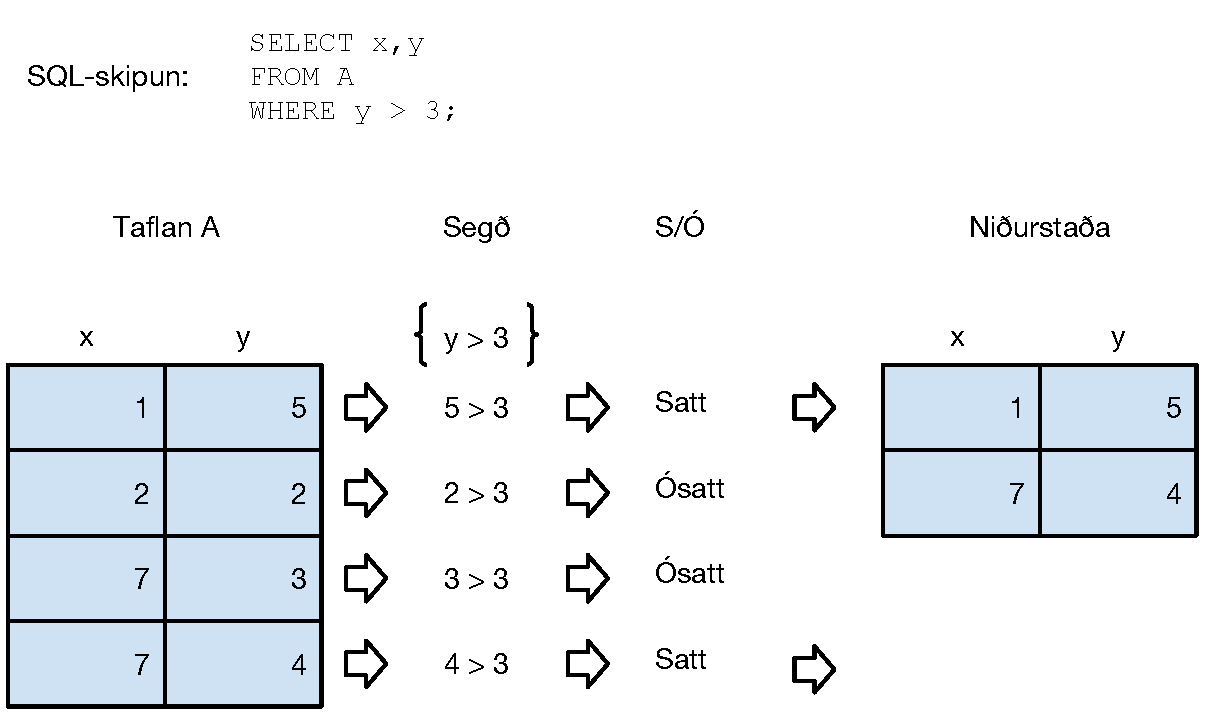
\includegraphics[width=\linewidth]{myndir/roksegd}
\end{figure}

Eins og við höfum t.d. séð á sýnidæmi \ref{sql:k4d6-where-nafn-endurtekid} þarf röksegð ekki að innihalda eingöngu samanburði með tölum. T.d. er hægt að bera saman strengi og dagsetningar.

Dagsetningar eru bornar saman líkt og tölur. Strengir eru hins vegar bornir saman í stafrófsröð\footnote{Þannig að stafurinn $a$ sé ``minni en'' stafurinn $b$.}. Dæmi um segðir sem innihalda strengi má sjá á töflu \ref{tafla:samanburdir-strengir}.

Nokkur atriði ber þó að varast þegar strengir eru notaðir til samanburðar í MySQL.

\newthought{Sérstakir stafir og tákn }á borð við upphrópunarmerki og bil eru ekki alltaf borin saman á þann hátt sem við giskum á. Stafrófsröð er ekki skilgreind fyrir þessi tákn. Pössum okkur þegar við notum $>$ eða $<$ til að bera saman strengi sem ekki innihalda eingöngu bókstafi.\footnote{Gagnlegt getur verið að lesa sér til um \emph{Collations} í MySQL til að öðlast frekari skilning á strengjasamanburðum. Ekki er fjallað um það í þessari bók.}

\newthought{Séu strengir af mismunandi lengdum bornir saman }er bilum bætt við hægra megin við styttri strenginn áður en samanburðurinn er framkvæmdur. Þannig myndi \verb|'a' > 'aa'| vera breytt í \verb|'a ' > 'aa'|. Þetta getur leitt til óvæntra niðurstaðna. Dæmi um niðurstöðu sem við fyrstu sýn kann að virðast undarleg má sjá á sýnidæmi \ref{sql:k4d7-where-nafn-staerra-en}.

\begin{table}
\centering
\caption[Röksegðir með strengjum]{Dæmi um hvernig MySQL meðhöndlar röksegðir með strengjum.}
\label{tafla:samanburdir-strengir}
\begin{tabular}{ll}
\toprule
Segð&Gildi\\
\midrule
\verb|'a' = 'a'|&Satt.\\
\verb|'a' >= 'a'|&Satt.\\
\verb|'b' > 'a'|&Satt, af því að $b$ er á eftir $a$ í stafrófinu.\\
\verb|'a' > 'b'|&Ósatt, af því að $b$ er á eftir $a$ í stafrófinu.\\
\verb|'ab' > 'aa'|&Satt, af því að aftari stafir útkljá jafntefli.\\
\verb|'a b' > 'a a'|&Satt, af því að bil er sagt minna en $a$.\\
\verb|'a b' > 'aaa'|&Ósatt, af því að bil er sagt minna en $a$.\\
\verb|'ab' > 'aabbb'|&Satt, af því að í samanburði mislangra strengja\\
&er bilum bætt við hægra megin við styttri strenginn.\\
\bottomrule
\end{tabular}
\end{table}

\begin{example}
\caption[Stærra-en samanburður við streng][-1.5cm]{\emph{SELECT}-skipun sem ber saman öll nöfn við strenginn \emph{'M'}. Skipunin skilar nöfnum allra nemanda sem eru á eftir \emph{M} í stafrófinu, \emph{að nemendum sem byrja á M meðtöldum!} Þetta er vegna þess að strengurinn \emph{M} er lengdur með bilum áður en samanburðurinn er framkvæmdur. Bil er álitið ``minna'' en allir bókstafir, svo segðin verður sönn fyrir öll nöfn sem byrja á \emph{M}.}
\label{sql:k4d7-where-nafn-staerra-en}
\centering
\sql{sql/k4d7-where-nafn-staerra-en.sql}
\end{example}

\subsection{LIKE og ``wildcards''}
Táknin sem við höfum séð í \verb|WHERE| klausum (t.d. $=$ og $>$) hafa gert okkur kleift að skrifa margar mismunandi röksegðir.

Ein gerð af segð sem við höfum ekki getað gert er að athuga hvort að strengur passi við hluta af öðrum streng. Til þess höfum við ákveðið lykilorð sem heitir \verb|LIKE|.

Það að nota \verb|LIKE| í röksegð er líkt og að nota \verb|=|. \verb|LIKE| hefur þó ákveðinn möguleika sem \verb|=| hefur ekki - þann að skilja eftir ``óþekkta'' stafi í strengnum sem notaður er til samanburðar. Þessi óvissutákn geta komið í stað hvaða stafs sem er. Þau eru kölluð ``wildcards'' á ensku. Við skoðum tvö mismunandi wildcards í þessum undirkafla. 

Annars vegar er táknið \verb|_| (strik niðri). \verb|_| getur komið í staðinn fyrir hvaða \emph{einn} staf sem er í strengnum.

Hins vegar er táknið \verb|%| (prósentumerki). \verb|%| getur komið í staðinn fyrir hvaða fjölda stafa sem er (líka fjöldann $0$).

Dæmi \ref{sql:k4d8-like-upphaf} til \ref{sql:k4d12-like-kennitala} sýna notkun \verb|LIKE| og wildcard-tákna.

\begin{example}
\caption[LIKE til að finna orð sem byrja á sama staf][-1.5cm]{\emph{SELECT} skipun sem finnur alla nemendur í nemendatöflunni sem byrja á stafnum \emph{K}. Til þess er notaður samanburðarstrengur sem hefur wildcard-táknið \emph{\%} á eftir stafnum \emph{K}, svo að \emph{\%} komi í staðinn fyrir allt sem á eftir \emph{K} kemur.}
\label{sql:k4d8-like-upphaf}
\centering
\sql{sql/k4d8-like-upphaf.sql}
\end{example}

\begin{example}
\caption[LIKE til að finna orð sem enda eins]{\emph{SELECT} skipun sem finnur alla nemendur í nemendatöflunni sem enda á \emph{``dóttir''}. \emph{\%} kemur hér á undan \emph{``dóttir''} svo að það geti komið í staðinn fyrir alla stafi sem gætu verið þar á undan.}
\label{sql:k4d9-like-lok}
\centering
\sql{sql/k4d9-like-lok.sql}
\end{example}

\begin{example}
\caption[LIKE einhvers staðar í streng]{\emph{SELECT} skipun sem finnur alla nemendur í nemendatöflunni sem innihalda strenginn ``geir'' einhvers staðar í nafni sínu. Segðin í \emph{WHERE}-klausunni er t.d. sönn fyrir nemandann sem heitir Ásgeir að millinafni og nemandann sem er Sigurgeirsson.}
\label{sql:k4d10-like-midja}
\centering
\sql{sql/k4d10-like-midja.sql}
\vspace{2cm}
\end{example}

\begin{example}
\caption[LIKE til að finna strengi af ákveðinni lengd]{\emph{SELECT} skipun sem finnur alla nemendur sem eru með nákvæmlega 17 stafi í nafni sínu (að bilum meðtöldum). Hvert \_ tákn kemur í stað nákvæmlega eins stafs. Við sjáum aðra leið til að gera þetta í undirkafla \ref{undirkafli:einindafoll}.}
\label{sql:k4d11-like-nakvaemt}
\centering
\sql{sql/k4d11-like-nakvaemt.sql}
\vspace{1cm}
\end{example}

\begin{example}
\caption[LIKE með nákvæmum stafafjölda]{\emph{SELECT} skipun sem finnur alla nemendur í nemendatöflunni sem fæddir eru í apríl (með stafina 04 í þriðja og fjórða sæti í kennitölu sinni). Hún finnur einungis þá nemendur, vegna þess að \_ táknin tvö geta komið í staðinn fyrir nákvæmlega tvö önnur tákn, hvorki fleiri né færri.}
\label{sql:k4d12-like-kennitala}
\centering
\sql{sql/k4d12-like-kennitala.sql}
\end{example}

\subsection{Mörg aðskilin skilyrði} % AND, OR
Hver \verb|SELECT| skipun getur einungis haft eina \verb|WHERE| klausu. Engu að síður er hægt að setja mörg skilyrði um þær raðir sem eiga að birtast í niðurstöðum skipunarinnar með því að tengja margar röksegðir saman. Það má gera með lykilorðunum \verb|AND| og \verb|OR|\footnote{Fleiri lykilorð af þessum toga eru til, til dæmis \emph{XOR}.}. Þannig mætti til dæmis búa til samsettu röksegðina \verb|x < 1 OR x > 5| úr segðunum \verb|x < 1|, \verb|x > 5| og lykilorðinu \verb|OR|.

\begin{marginfigure}
\caption[Samsett röksegð]{Hér sést hvernig lesa má út úr samsettri röksegð.}
\label{mynd:samsett-segd}
\centering
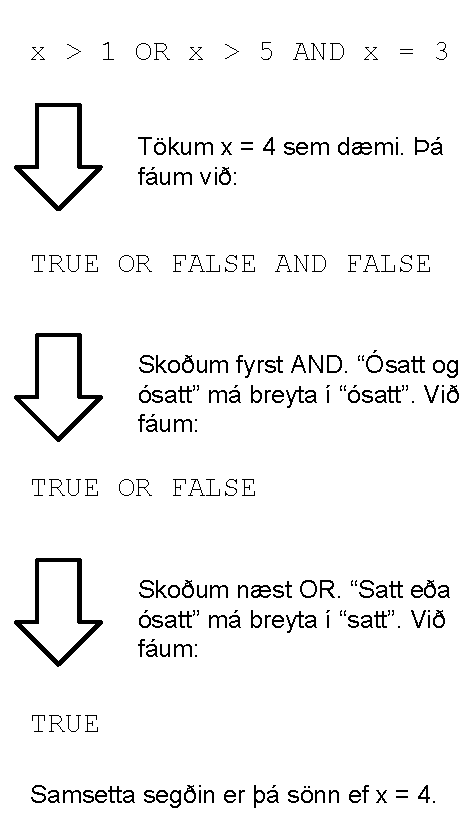
\includegraphics[width=\linewidth]{myndir/samsett-segd}
\end{marginfigure}

Þegar skoða á hvort að samsett segð sé sönn eða ósönn þarf fyrst að athuga hvort að segðirnar sem hún er búin til úr séu sannar eða ósannar. Þá verður úr röð af gildunum ``satt'' og ``ósatt'', með \verb|AND| og \verb|OR| á milli. 

Næst þarf að athuga öll \verb|AND| í röðinni. Þegar \verb|AND| stendur á milli tveggja gilda sem eru sönn mynda þau saman gildið ``satt'', annars gildið ``ósatt''. Þegar \verb|AND| stendur á milli tveggja gilda þurfa sem sagt bæði gildin að vera sönn til að útkoman sé sönn.

Að lokum eru öll \verb|OR| skoðuð. Þegar \verb|OR| stendur á milli tveggja gilda er nóg að annað gildanna sé ``satt'' til að þau myndi saman gildið ``satt''. Séu bæði gildin ósönn mynda þau gildið ``ósatt''.

\begin{table}[b]
\caption[AND og OR]{Hér sést hvaða áhrif það hefur að setja \emph{AND} og \emph{OR} á milli tveggja breyta. Gildi breytanna er í vinstri dálkunum, útkoman sést í dálkunum til hægri.}
\label{tafla:and-or}
\centering
\begin{tabular}{ccc}
\multicolumn{3}{c}{Útkoma \emph{AND}}\\
\toprule
$x$&$y$&$x$ \emph{AND} $y$\\
\midrule
1&1&1\\
1&0&0\\
0&1&0\\
0&0&0\\
\bottomrule
\end{tabular}
\hspace{1cm}
\begin{tabular}{ccc}
\multicolumn{3}{c}{Útkoma \emph{OR}}\\
\toprule
$x$&$y$&$x$ \emph{OR} $y$\\
\midrule
1&1&1\\
1&0&1\\
0&1&1\\
0&0&0\\
\bottomrule
\end{tabular}
\end{table}

\newthought{Allt þetta tal} um segðir og samsetningar kann að hljóma þurrt. Þetta á sér þó hliðstæður í mun raunverulegri aðstæðum.

Skoðum dæmi \ref{sql:k4d8-like-upphaf} og \ref{sql:k4d9-like-lok} aftur. Í fyrra dæminu finnum við alla nemendur sem heita nafni sem byrjar á bókstafnum \emph{``K''}, í seinna dæminu finnum við alla nemendur sem heita nafni sem endar á \emph{``dóttir''}. Viljum við finna alla nemendur með nafn sem bæði byrjar á \emph{``K''} og endar á \emph{``dóttir''} getum við tengt skilyrðin tvö saman. Úr verður \verb|WHERE| klausan í sýnidæmi \ref{sql:k4d13-where-and}.

\verb|OR| kemur fyrir þegar einungis eitt af tveimur skilyrðum þarf að vera uppfyllt. Lítum aftur á dæmi \ref{sql:k4d12-like-kennitala}, þar sem allir nemendur sem fæddir eru í apríl eru valdir. Vildum við breyta skipuninni svo að hún myndi ná í alla nemendur sem fæddir eru annaðhvort í apríl eða í júní gætum við notað \verb|OR| á svipaðan hátt og gert er í dæmi \ref{sql:k4d14-where-or}.

\begin{example}
\caption[WHERE með AND]{\emph{SELECT} skipun sem finnur alla nemendur í nemendatöflunni sem heita nafni sem bæði byrjar á \emph{``K''} og endar á \emph{``dóttir''}.}
\label{sql:k4d13-where-and}
\centering
\sql{sql/k4d13-where-and.sql}
\end{example}

\begin{example}
\caption[WHERE með OR]{\emph{SELECT} skipun sem finnur alla nemendur í nemendatöflunni sem fæddir eru í apríl eða júní.}
\label{sql:k4d14-where-or}.
\centering
\sql{sql/k4d14-where-or.sql}
\end{example}

\newpage
Freistandi getur verið að skrifa \verb|WHERE| klausur þar sem mörg samanburðar\emph{gildi} eru talin upp hvert af öðru, tengd með \verb|AND| eða \verb|OR|. Þetta gengur ekki! Munum alltaf að það eru röksegðir sem \verb|AND| og \verb|OR| tengja saman, það að reyna að nota þau til að tengja saman almenna strengi eða tölur getur leitt til óvæntra niðurstaðna. \footnote{Dæmi um þessa villu væri t.d. að skrifa \emph{WHERE x = 1 OR 3} til að finna línurnar þar sem $x$ er $1$ eða $3$. Rétt væri að skrifa \emph{WHERE x = 1 OR x = 3}.}

Munum líka að \verb|OR| í röksegð er ekki alveg það sama og ``eða'' í talmáli. Í talmáli þýðir ``eða'' oft val á milli tveggja möguleika (má bjóða þér salat eða franskar með hamborgaranum?) en í röksegðum skilar samsett segð sönnu svo lengi sem annar ``möguleikinn'' á við. \footnote{Um þetta er til gamall brandari.

Eiginmaður tölvunarfræðings spyr: ``Langar þig í fisk eða kjöt í kvöldmat?'' Tölvunarfræðinginn langar í kjöt, svo hún svarar: ``Já.''}
\subsection{Að velja úr mengi - IN} %IN
Oft þarf að gera mjög marga samanburði í \verb|WHERE| klausu. Þá getur orðið flókið að koma skilyrðunum fyrir.

Hægt er að gera suma samanburði (sérstaklega þá sem annars þyrftu mörg \verb|OR| skilyrði) einfaldari með því að nota lykilorðið \verb|IN|. Segð sem inniheldur \verb|IN| ber saman gildi við ``mengi'' gilda og skilar sönnu ef samanburðargildið er í menginu. \footnote{\emph{IN} getur verið sérstaklega gagnlegt þegar undirfyrirspurnir koma við sögu. Sjá kafla \ref{undirkafli:undirfyrirspurnir}.}

Dæmi um notkun \verb|IN| má sjá á sýnidæmi \ref{sql:k4d15-where-in}.

\begin{example}
\caption[WHERE með IN]{Tvær \emph{SELECT} skipanir sem gera sama hlutinn. Þær finna báðar nemendurna með númerin 1, 3, 5 og 7. Seinni skipunin er þó töluvert skárri!}
\label{sql:k4d15-where-in}.
\centering
\sql{sql/k4d15-where-in.sql}
\end{example}
\subsection{Að snúa við skilyrði - NOT}
Merkingu flestra röksegða má snúa við með því að setja lykilorðið \verb|NOT| fyrir framan segðina. Hafi segðin áður skilað sönnu skilar hún þess í stað ósönnu, hafi hún skilað ósönnu skilar hún sönnu. Dæmi um notkun \verb|NOT| má sjá á sýnidæmi \ref{sql:k4d16-not}.

\begin{example}
\caption[NOT lykilorðið]{\emph{SELECT} skipun sem finnur alla nemendur sem \emph{ekki} byrja á stafnum \emph{``K''}.}
\label{sql:k4d16-not}.
\centering
\sql{sql/k4d16-not.sql}
\end{example}
\section{Um föll}
\label{undirkafli:foll}
Fall\footnote{e. \emph{function}} er mikilvægt stærðfræðihugtak sem kemur víða við í forritun, þar á meðal í SQL.

Líta má á fall sem nokkurns konar ``vél'' sem breytir einu í annað. Fall \emph{tekur eitthvað inn} og \emph{skilar} einhverju öðru.

\begin{marginfigure}
\caption[Fall]{Líta má á fall $f$ sem vél sem breytir gildinu $x$ í gildið $f(x)$.}
\label{mynd:fall}
\centering
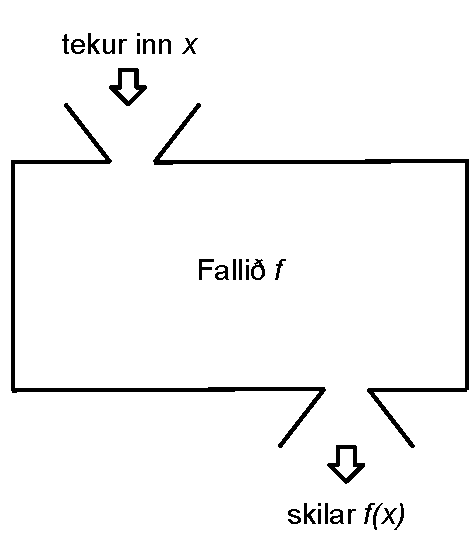
\includegraphics[width=\linewidth]{myndir/fall}
\end{marginfigure}

Við getum t.d. litið á brauðrist sem fall. Brauðrist \emph{tekur inn} brauð og \emph{skilar} ristuðu brauði. Á stærðfræðimáli myndum við skrifa það svona:
\[
\text{brauðrist(brauð)} = \text{ristað brauð}
\]

\section{Helstu ``scalar'' föll}
\label{undirkafli:einindafoll}
Í þessum undirkafla ætlum við að skoða MySQL-föll sem taka inn eitt eða ekkert gildi og skila einu gildi. Þau eru kölluð ``scalar föll''. Ekki er til íslenskt orð yfir hugtakið sem er í almennri notkun.
\subsection{Lengd strengs - CHAR\_LENGTH}
Fyrsta fallið sem við skoðum er MySQL-fallið \verb|CHAR_LENGTH|. Það fall tekur inn streng og skilar fjölda stafa sem er í strengnum. Bil og önnur tákn eru tekin með. Almenn lýsing á fallinu gæti þá verið svona:
\[
\text{CHAR\_LENGTH(texti)} = \text{fjöldi stafa í texta}
\]
Og dæmi um notkun (á stærðfræðiformi)
\[
\text{CHAR\_LENGTH('Jónas')} = 5
\]

Notkun fallsins í MySQL má sjá í sýnidæmi \ref{sql:k4d17-char-length}.

\begin{example}[h]
\caption[CHAR\_LENGTH]{\emph{SELECT} skipun sem finnur fjölda stafa í orðinu ``Jónas'' með \emph{CHAR\_LENGTH} fallinu. Þessi skipun skilar sem sagt tölunni 5.}
\label{sql:k4d17-char-length}
\centering
\sql{sql/k4d17-char-length.sql}
\end{example}

Annað fall, sem heitir einfaldlega \verb|LENGTH|, er líka til. Það fall skilar fjölda bæta sem eru í strengnum. Oft er einn bókstafur geymdur í einu bæti, svo \verb|LENGTH| og \verb|CHAR_LENGTH| skila oft sömu tölu, en munur getur komið fram þegar bókstafir eru geymdir í meira en einu bæti. Séríslenskir stafir eru t.d. venjulega geymdir í tveimur bætum. \verb|LENGTH('Jónas')| myndi þess vegna skila tölunni $6$. 

% \subsection{ROUND} 
\subsection{UCASE og LCASE}
\verb|UCASE| er fall sem tekur inn streng og skilar honum í hástöfum. \verb|UCASE| er stytting á enska orðinu ``uppercase''. Notkun fallsins í MySQL má sjá í sýnidæmi \ref{sql:k4d18-ucase}.

\begin{example}[h]
\caption[UCASE]{\emph{SELECT} skipun sem skilar strengnum ``JÓNAS''.}
\label{sql:k4d18-ucase}
\centering
\sql{sql/k4d18-ucase.sql}
\end{example}

Fallinu má lýsa á eftirfarandi hátt:
\[
\text{UCASE(textinn)} = \text{textinn í hástöfum}
\]
Dæmi um notkun er:
\[
\text{UCASE('Jónas')} = \text{'JÓNAS'}
\]

\verb|LCASE| er svipað fall. Það fall tekur inn streng og skilar honum í lágstöfum. \verb|LCASE| er stytting á orðinu ``lowercase''.
\subsection{NOW}
\verb|NOW| er fall sem skilar núverandi tímasetningu (skv. klukku MySQL-serversins). \verb|NOW| er ólíkt föllunum hér á undan að því leytinu til að það þarf ekki að taka neitt inn, það skilar bara gildi (þessi vél þarf ekkert hráefni!).

Til að prenta núverandi tímasetningu út mætti sem sagt einfaldlega keyra skipunina \verb|SELECT NOW();|.\footnote{Þó að \emph{NOW} fallið taki ekkert inn þurfa svigarnir samt að vera til staðar. Svigarnir segja MySQL að um fall sé að ræða.}
\subsection{Notkun scalar falla}
Föllin sem við höfum farið yfir eru sjaldnast notuð ein og sér. Oftast eru þau notuð á eftirfarandi vegu:
\begin{enumerate}
 \item Sem hluti af lýsingu á því hvaða dálka \verb|SELECT| skipun á að ná í.
 \item Sem hluti af \verb|WHERE| klausu, til samanburðar við gildi.
\end{enumerate}

Fyrri notkunina má sjá í sýnidæmi \ref{sql:k4d19-char-length-haus}. Þar er allur dálkurinn \emph{nafn} settur inn í \verb|CHAR_LENGTH| fallið.

Áðan sögðum við að \verb|CHAR_LENGTH| taki aðeins við einum streng. Þegar heill dálkur er settur inn í fall sem einungis tekur við einum streng (scalar fall) er fallið notað á hverja línu í dálkinum, eina í einu. Niðurstöðurnar birtast þá sem heill dálkur líka, líkt og sjá má á töflu \ref{tafla:lengd-nafna}.

\begin{example}
\caption[CHAR\_LENGTH í dálklýsingu]{\emph{SELECT} skipun sem finnur lengd nafna allra nemenda í nemendatöflunni sem enda á \emph{``dóttir''}. Niðurstöðu má sjá á töflu \ref{tafla:lengd-nafna}.}
\label{sql:k4d19-char-length-haus}
\centering
\sql{sql/k4d19-char-length-haus.sql}
\end{example}

\begin{table}
\centering
\caption[Lengd nafna]{Niðurstaða sýnidæmis \ref{sql:k4d19-char-length-haus}.}
\label{tafla:lengd-nafna}
\begin{tabular}{ll}
\toprule
\verb|nafn|&\verb|CHAR_LENGTH(nafn)|\\
\midrule
Ingunn Rún Andradóttir&22\\
Pálína Björk Þórólfsdóttir&26\\
Regína Sigrún Jensdóttir&24\\
Líney Geirsdóttir&17\\
Steinunn Berglind Eiðsdóttir&28\\
Kristjana Ólafsdóttir&21\\
Þóra Gestsdóttir&16\\
Kolfinna Svava Óttarsdóttir&27\\
Elísabet Hrannarsdóttir&23\\
Hafrún Þorláksdóttir&20\\
\bottomrule
\end{tabular}
\end{table}

Seinni notkunina má sjá í sýnidæmi \ref{sql:k4d20-char-length-where}. Þar er fallið \verb|CHAR_LENGTH| notað í \verb|WHERE| klausu. Reiknað er upp úr fallinu fyrir hverja línu og útkoman borin saman við tölu.

\begin{example}
\caption[CHAR\_LENGTH í WHERE klausu]{\emph{SELECT} skipun sem finnur nöfn allra nemenda sem heita sextán stafa nafni (að bilum meðtöldum).}
\label{sql:k4d20-char-length-where}
\centering
\sql{sql/k4d20-char-length-where.sql}
\end{example}

\section{GROUP BY}
Hingað til höfum við unnið með hrá gögn eins og þau koma fram í upphaflegu töflunni. Hver lína í niðurstöðunum samsvarar nákvæmlega einni línu í töflunni sem valið er úr.

En þetta dugar okkur ekki alltaf. Stundum þurfum við að geta litið á margar línur í einu.

Til þess að skoða margar línur í einu er \verb|GROUP BY| klausan gagnleg. Hún tekur töfluna sem valið er úr og skiptir henni í ``hópa''.

Hópar af línum eru búnir til út frá sameiginlegum atriðum. Þessi ``sameiginlegu atriði'' eru gildi í einum eða fleiri dálkum. 

Einföld \verb|GROUP BY| klausa tekur sem sagt við nafni á dálki og setur allar línur sem hafa sama gildið í þeim dálki saman í hóp. Dæmi um hvernig svona skipting gæti gengið fyrir sig má sjá á mynd \ref{mynd:group-by}.

\begin{figure}
\caption[GROUP BY]{Sýnir hvernig GROUP BY klausa gæti skipt töflu upp í hópa eftir því hvaða gildi er í dálkinum $y$.}
\label{mynd:group-by}
\centering
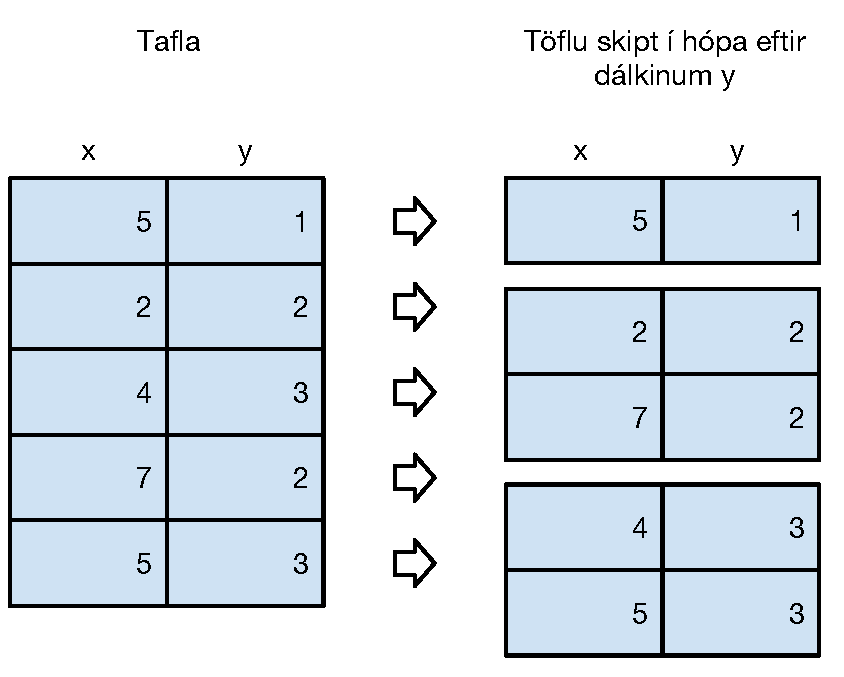
\includegraphics[width=\linewidth]{myndir/group-by}
\end{figure}

Mikilvægt er að átta sig á að þegar \verb|GROUP BY| klausa er til staðar í \verb|SELECT| skipun samanstanda niðurstöðurnar ekki af línum, heldur \emph{hópum} af línum. Klausan breytir eðli skipunarinnar. 

\section{Samsteypuföll}
Föllin sem við höfum skoðað hingað til hafa ekki tekið inn meira en eitt gildi í einu. Nú lítum við á föll sem geta tekið inn fjöldann allan af gildum og unnið með þau sem eina heild. Slík föll eru kölluð samsteypuföll\footnote{e. \emph{aggregate function}}.

Samsteypuföll í MySQL geta sem sagt tekið inn mengi af gildum og skilað svo upplýsingum um mengið. Mengið getur verið heill dálkur eða ``hópur'' af gildum sem \verb|GROUP BY| klausa býr til.

\subsection{COUNT}
Mest notaða samsteypufallið er líklega fallið \verb|COUNT|. \verb|COUNT| tekur inn mengi af gildum og skilar fjölda þeirra - fallið telur stökin.

Til að kynnast \verb|COUNT| aðeins betur skulum við byrja á að skoða nýja töflu, töflu \ref{tafla:afangar}.

\begin{table}
\centering
\caption[Áfangar]{Áfangar grunndeildar tölvubrautar Tækniskólans. Í töflunni eru upplýsingar um auðkenni áfangans (nafn hans), fagið sem áfangarnir tilheyra, og önnina sem þeir eru kenndir á. Dálkurinn \emph{numer} er aðallykill.}
\label{tafla:afangar}
\begin{tabular}{llll}
\toprule
numer&audkenni&fag&onn\\
\midrule
1&	FOR1A3U&	Forritun&		1\\
2&	VSH1A3U&	Vefhönnun&		1\\
3&	GSÖ1G2U&	Notkun gagnasafna&	1\\
4&	TÆK1A1U&	Tölvutækni&		1\\
5&	FOR1B3U&	Forritun&		2\\
6&	VSH2A3U&	Vefhönnun&		2\\
7&	GSÖ1F2U&	Notkun gagnasafna&	2\\
8&	TÆK2A3U&	Tölvutækni&		2\\
9&	FOR2B2U&	Forritun&		3\\
10&	VSH2B2U&	Vefhönnun&		3\\
11&	GSÖ2B2U&	Notkun gagnasafna&	3\\
12&	TÆK2B2U&	Tölvutækni&		3\\
13&	GRU2L4U&	Lokaverkefni grunndeildar&3\\
\bottomrule
\end{tabular}
\end{table}

Við getum t.d. notað \verb|COUNT| fallið til að komast að því hversu margir áfangar eru í grunndeildinni. Slíka skipun má sjá á sýnidæmi \ref{sql:k4d21-count}.

\begin{example}
\caption[COUNT á dálk]{\emph{SELECT} skipun sem finnur fjölda lína í \emph{Afangar} töflunni (töluna 13). Í raun er fjöldi gilda í dálkinum \emph{numer} talinn, en þar sem við vitum að \emph{numer} er aðallykill getum við verið viss um að allar línurnar séu taldar.}
\label{sql:k4d21-count}
\centering
\sql{sql/k4d21-count.sql}
\end{example}

Sé \verb|COUNT| notað með \verb|GROUP BY| klausu er ekki allur dálkurinn talinn, heldur er fjöldi staka (eða lína) í hverjum hópi talinn fyrir sig. Dæmi um slíka skipun og hvernig niðurstöður hennar geta litið út má sjá á myndum \ref{mynd:workbench-group-by} og \ref{mynd:workbench-group-by-onn}.

\begin{figure*}
\caption[GROUP BY og COUNT eftir fögum]{Dæmi um \emph{SELECT} skipun með \emph{GROUP BY} klausu sem raðar áföngum saman í hópa eftir því hvaða fagi þeir tilheyra. Síðan telur \emph{COUNT} hversu margir áfangar tilheyra hverju fagi.}
\label{mynd:workbench-group-by}
\centering
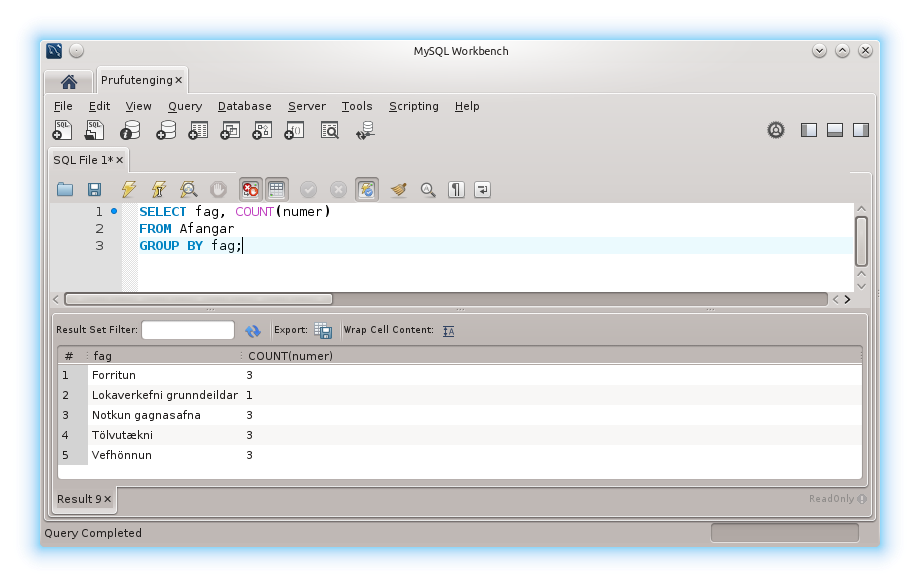
\includegraphics[width=\linewidth]{myndir/workbench-group-by}
\end{figure*}

\begin{figure*}
\caption[GROUP BY og COUNT eftir önnum]{Dæmi um \emph{SELECT} skipun með \emph{GROUP BY} klausu sem raðar áföngum saman í hópa eftir því hvaða önn þeir eru kenndir á. Síðan telur \emph{COUNT} hversu margir áfangar eru á hverri önn.}
\label{mynd:workbench-group-by-onn}
\centering
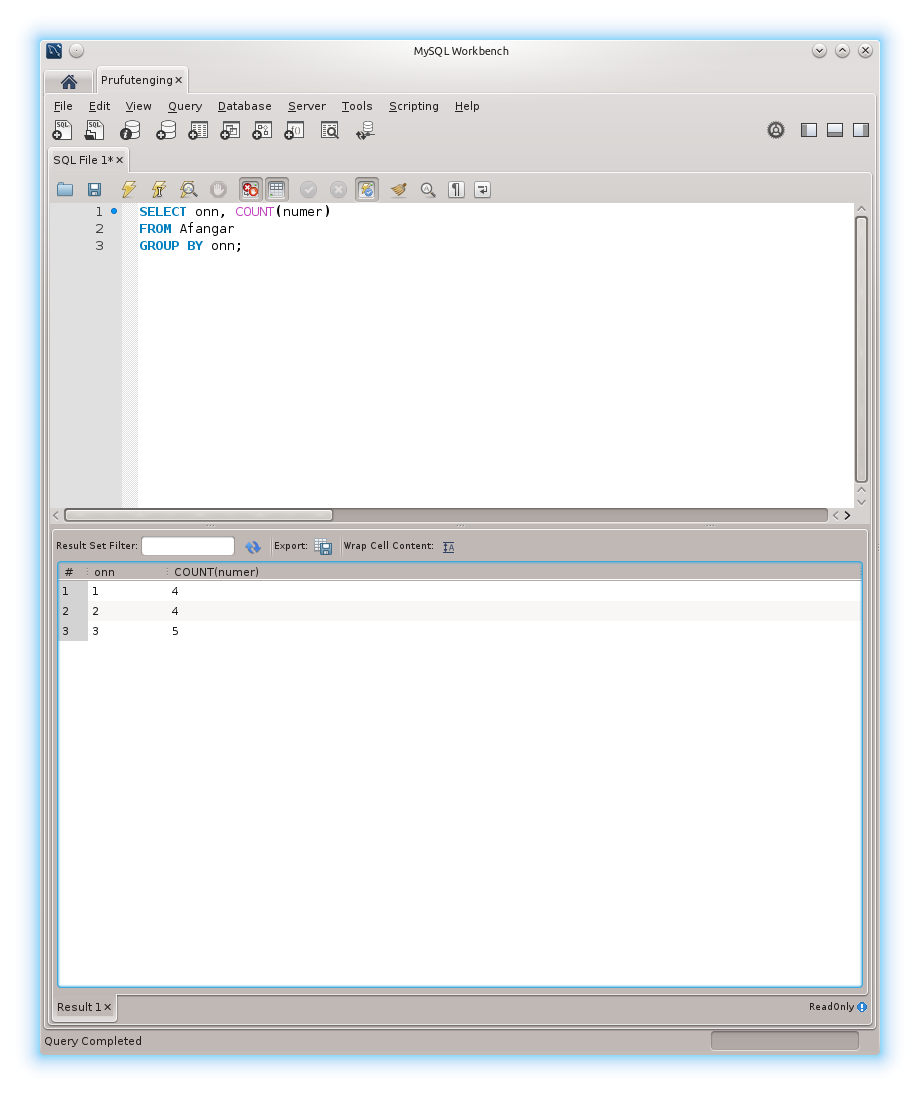
\includegraphics[width=\linewidth]{myndir/workbench-group-by-onn-stort}
\end{figure*}

\newpage
\subsection{Önnur samsteypuföll - MIN, MAX, SUM, og AVG}
\label{undirkafli:onnur-samsteypufoll}
Fleiri samsteypuföll eru til en \verb|COUNT|. Lítum á nokkur til viðbótar. Öll eiga þau sameiginlegt að taka inn mengi af gildum og skila okkur upplýsingum um mengið sjálft.

\begin{itemize}
 \item \verb|MIN| tekur inn mengi og skilar minnsta stakinu í menginu.
 \item \verb|MAX| tekur inn mengi og skilar stærsta stakinu í menginu.
 \item \verb|SUM| tekur inn mengi og skilar summu staka í menginu.
 \item \verb|AVG| tekur inn mengi og skilar meðaltali staka í menginu.
\end{itemize}

Þau eru notuð á svipaðan hátt og \verb|COUNT|. Skoðum enn aðra töflu, töflu \ref{tafla:einkunnir}, til að kynnast þeim betur.

\begin{table}
\centering
\caption[Einkunnir]{Nokkrir nemendur og einkunnir þeirra.}
\label{tafla:einkunnir}
\begin{tabular}{llr}
\toprule
numer&nafn&einkunn\\
\midrule
1&Birgir Torfason&5.5\\
2&Höskuldur Frímann Ásmundsson&3.0\\
3&Jón Guðmundsson&9.0\\
4&Hilmar Hjartarson&5.0\\
5&Reynir Rafn Sigurgeirsson&8.0\\
6&Ingunn Rún Andradóttir&10.0\\
7&Pálína Björk Þórólfsdóttir&3.5\\
8&Regína Sigrún Jensdóttir&1.5\\
9&Líney Geirsdóttir&2.5\\
10&Steinunn Berglind Eiðsdóttir&4.0\\
\bottomrule
\end{tabular}
\end{table}

Við getum notað samsteypuföll til að fá frekari upplýsingar um töfluna. Sjá sýnidæmi \ref{sql:k4d28-min} og \ref{sql:k4d29-avg}.

\begin{example}
\caption[MIN fallið]{\emph{SELECT} skipun sem finnur lægstu einkunnina í einkunnatöflunni. Hún finnur gildið $1.5$. 

\emph{Athugum þó} að ekki væri hægt að finna hver hefur þá einkunn með því að skrifa \emph{SELECT nafn, MIN(einkunn)}. \emph{MIN} er samsteypufall sem vinnur (hér) með dálkinn \emph{einkunn} í heild sinni, það veit ekki af öðrum dálkum. Undirkaflar \ref{undirkafli:having} og \ref{undirkafli:undirfyrirspurnir} sýna dæmi um vinnslu með samsteypuföll.}
\label{sql:k4d28-min}
\centering
\sql{sql/k4d28-min.sql}
\end{example}

\clearpage
\begin{example}
\caption[AVG fallið]{\emph{SELECT} skipun sem finnur meðaleinkunnina í einkunnatöflunni. Hún finnur gildið $5.2$.}
\label{sql:k4d29-avg}
\centering
\sql{sql/k4d29-avg.sql}
\end{example}

\section{HAVING}
\label{undirkafli:having}
Við vorum búin að komast að því að \verb|GROUP BY| klausa breytir eðli \verb|SELECT| skipunar sem hún tilheyrir. Niðurstöður skipunar sem inniheldur \verb|GROUP BY| klausuna eru nefnilega hópar af línum (hóplínur), ekki línur.

Þetta hefur nokkrar afleiðingar í för með sér. Sérstaklega er sú afleiðing áberandi að \verb|WHERE| klausan virkar ekki sem fyrr. \verb|WHERE| klausan vinnur með línur, hún getur ekki unnið með hóplínur.

Til þess að sía burt hóplínur þarf að nota enn aðra klausu - \verb|HAVING|. \verb|HAVING| virkar eins og \verb|WHERE| klausan, nema hún vinnur með hóplínur. 

\verb|HAVING| klausuna má sjá á sýnidæmi \ref{sql:k4d22-having}.

\begin{example}
\caption[HAVING]{\emph{SELECT} skipun með \emph{HAVING} klausu sem finnur öll fög með þrjá áfanga. Væri reynt að nota \emph{WHERE} klausu hér í stað \emph{HAVING} myndi það leiða til villu!}
\label{sql:k4d22-having}
\centering
\sql{sql/k4d22-having.sql}
\end{example}

Yfirlit yfir það hvernig \verb|WHERE| og \verb|HAVING| virka saman má sjá á mynd \ref{mynd:group-by-having}. Myndin sýnir líka í hvaða röð \verb|FROM|, \verb|WHERE|, \verb|GROUP BY| og \verb|HAVING| klausurnar koma fyrir í \verb|SELECT| skipunum.
\begin{figure}
\caption[FROM, WHERE, GROUP BY og HAVING]{Lýsing á því hvernig FROM, WHERE, GROUP BY og HAVING klausurnar vinna saman.}
\label{mynd:group-by-having}
\centering
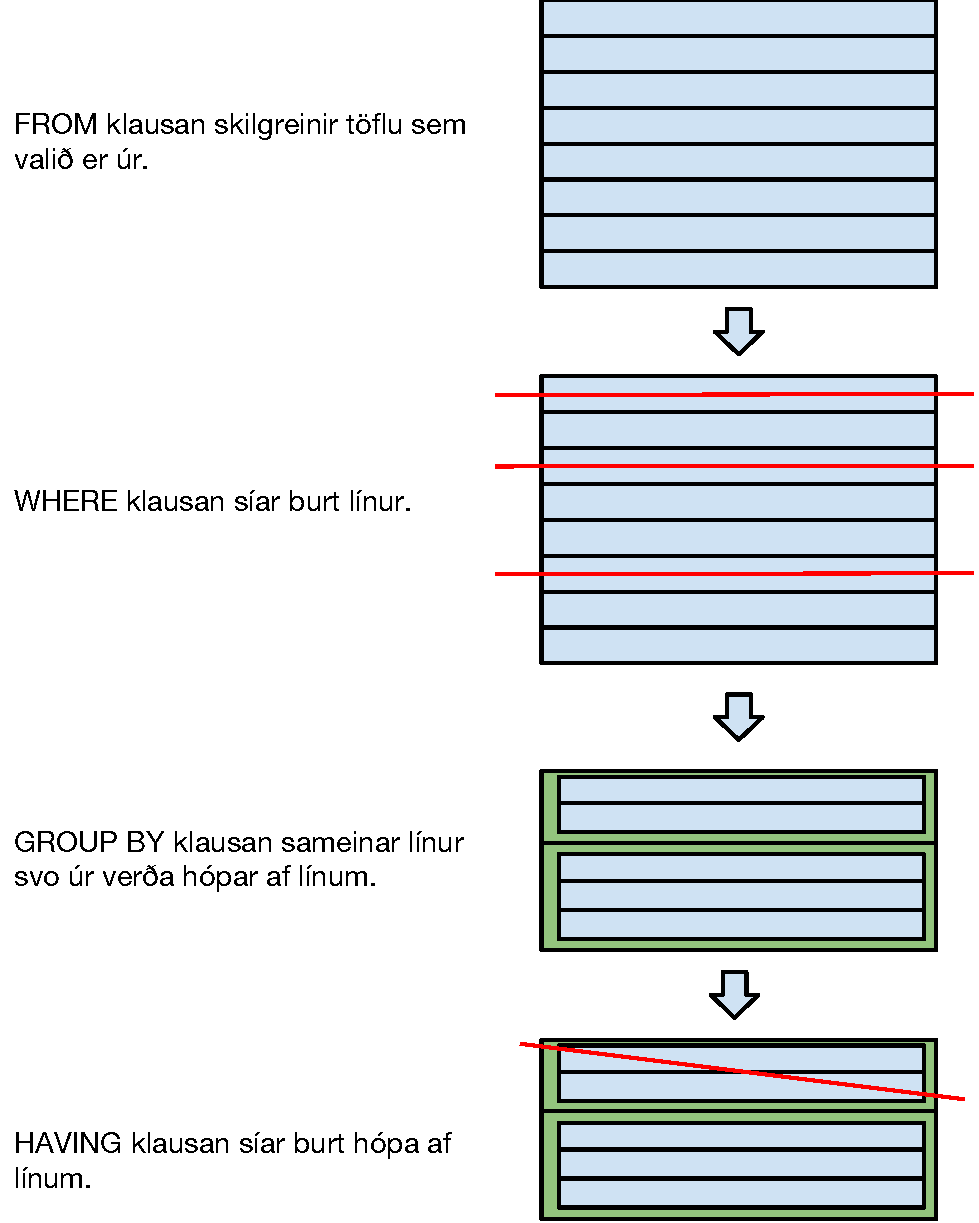
\includegraphics[width=\linewidth]{myndir/group-by-having}
\end{figure}

\section{ORDER BY}
Niðurstöður \verb|SELECT| skipananna sem við höfum séð hafa ekki birst í neinni sérstakri röð. Þær hafa birst í þeirri röð sem þær eru geymdar í í gagnagrunninum.\footnote{Þetta er oftast innsetningarröð gagnanna. Ekki er samt alltaf hægt að treysta á það.}

Til að láta gögnin birtast í ákveðinni röð má nota klausu sem heitir \verb|ORDER BY|. \verb|ORDER BY| klausan tekur við nafni á a.m.k. einum dálki og raðar línunum í röð eftir gildunum í þeim dálki.

Hægt er að raða línum eftir tölum, bókstöfum, dagsetningum, hverju sem er sem hægt er að bera saman.\footnote{Hér getur verið gott að rifja upp samanburði með röksegðum úr undirkafla \ref{undirkafli:roksegdir}.}

Sé annað ekki tekið fram er línunum raðað í hækkandi röð. ``Lægstu'' gildin koma fremst í röðinni, ``hæstu'' gildin koma aftast. Röðinni má snúa við með því að bæta lykilorðinu \verb|DESC| fyrir aftan dálkupptalninguna í \verb|ORDER BY| klausunni.

Notkun \verb|ORDER BY| klausunnar má sjá á sýnidæmum \ref{sql:k4d23-order-by} til \ref{sql:k4d25-order-by-tveir}.

\begin{example}
\caption[ORDER BY]{\emph{SELECT} skipun sem velur nemendur úr töflunni í stafrófsröð eftir nafni með því að nota \emph{ORDER BY} klausu.}
\label{sql:k4d23-order-by}
\centering
\sql{sql/k4d23-order-by.sql}
\end{example}

\begin{example}
\caption[ORDER BY með DESC]{\emph{SELECT} skipun sem velur nemendur úr töflunni í öfugri stafrófsröð.}
\label{sql:k4d24-order-by-desc}
\centering
\sql{sql/k4d24-order-by-desc.sql}
\end{example}

\begin{example}
\caption[ORDER BY með tveimur dálkum]{\emph{SELECT} skipun sem sýnir áfanga, fyrst raðaða eftir önninni sem þeir eru kenndir á, svo er stafrófsröð notuð til að raða áföngunum innbyrðis innan annanna.}
\label{sql:k4d25-order-by-tveir}
\centering
\sql{sql/k4d25-order-by-tveir.sql}
\end{example}
\section{LIMIT}
Stundum þurfum við ekki allar upplýsingarnar úr töflu. Til að takmarka hversu margar línur birtast í niðurstöðu \verb|SELECT| skipunar má nota síðustu klausuna sem við förum yfir í þessari bók - \verb|LIMIT|.

\verb|LIMIT| klausan tekur við einni eða tveimur tölum. 

Fái \verb|LIMIT| klausan eina tölu mun \verb|SELECT| skipunin einungis sýna þann fjölda af línum í niðurstöðunni. Fyrstu línurnar úr niðurstöðunni eru valdar. Þannig myndi t.d. \verb|LIMIT 5| sía allar línur úr niðurstöðunni nema þær fimm fyrstu.

Fái \verb|LIMIT| klausan tvær tölur skilar \verb|SELECT| skipunin ekki (endilega) fyrstu línunum úr niðurstöðunni. Klausan byrjar þá að telja á því línunúmeri sem fyrri talan segir til um, sú seinni segir til um hversu margar tölur eru valdar. Línunúmerin byrja að telja frá núlli. Þannig myndi t.d. \verb|LIMIT 5,10| hleypa í gegn línum $6-15$ og \verb|LIMIT 0,5| myndi gera það sama og \verb|LIMIT 5|.

Sýnidæmi \ref{sql:k4d26-limit} og \ref{sql:k4d27-limit-tveir} sýna notkun \verb|LIMIT| klausunnar.

\begin{example}
\caption[LIMIT]{\emph{SELECT} skipun sem velur þá þrjá nemendur sem fremstir eru í stafrófsröðinni. Niðurstöðunum raðað með \emph{ORDER BY}, síðan er öllum línum eftir þá þriðju hent með \emph{LIMIT} klausunni.}
\label{sql:k4d26-limit}
\centering
\sql{sql/k4d26-limit.sql}
\end{example}

\begin{example}
\caption[LIMIT með tveimur tölum]{\emph{SELECT} skipun sem velur nemanda númer 11 í stafrófsröðinni.}
\label{sql:k4d27-limit-tveir}
\centering
\sql{sql/k4d27-limit-tveir.sql}
\end{example}
\section{Uppbygging SELECT skipunarinnar}
Við höfum farið yfir fjölmargar klausur sem tilheyra \verb|SELECT| skipuninni.

Það skiptir máli í hvaða röð þessar klausur koma fram í \verb|SELECT| skipun. Þær þurfa að koma fram í nákvæmlega þeirri röð sem við kynntum þær. Sú röð er:

\begin{enumerate}
 \setcounter{enumi}{0}
 \item Haus \verb|SELECT| skipunarinnar
 \item \verb|FROM|
 \item \verb|WHERE|
 \item \verb|GROUP BY|
 \item \verb|HAVING|
 \item \verb|ORDER BY|
 \item \verb|LIMIT|
\end{enumerate}

Sleppa má hverri af klausunum sem er\footnote{\emph{HAVING} er þó mjög sjaldan notuð án \emph{GROUP BY}. Ekki er hægt að sleppa sjálfu \emph{SELECT} lykilorðinu.}. Þetta breytir ekki röðinni - \verb|WHERE| þarf alltaf að koma á eftir \verb|FROM|, \verb|ORDER BY| þarf alltaf að koma á eftir \verb|GROUP BY|, og svo framvegis. Almennt getur \verb|SELECT| skipun með þeim atriðum sem við höfum kynnst því litið út á þann hátt sem sjá má á sýnidæmi \ref{sql:k4d30-skema}.

\begin{example}
\caption[Uppbygging]{Uppbygging \emph{SELECT} skipunar með þeim atriðum sem koma fyrir í þessum (kafla \ref{kafli:select}).}
\label{sql:k4d30-skema}
\centering
\sql{sql/k4d30-skema.sql}
\end{example}

\newpage
\section{Yfirlit}
Í þessum kafla fórum við yfir \verb|SELECT| skipunina í MySQL.
\begin{itemize}
 \item \verb|SELECT| skipun er notuð til að ná í upplýsingar.
 \item Þegar \verb|FROM| klausa fylgir \verb|SELECT| skipun er klausan notuð til að skilgreina hvaðan upplýsingarnar koma. 
 \item \verb|WHERE| klausan síar burt upplýsingar frá \verb|FROM| klausunni. Til þess eru notaðir samanburðir.
 \begin{itemize}
  \item Hægt er að nota alls kyns samanburði í \verb|WHERE| klausu svo lengi sem samanburðurinn einfaldast niður í ``satt'' eða ``ósatt''.
 \end{itemize}
 \item Scalar föll í MySQL taka inn eitt eða ekkert gildi og skila einu gildi. Sé dálkur af gildum settur inn í scalar fall sem tekur við einu gildi er fallið notað á hvert gildi í dálkinum fyrir sig.
 \item \verb|GROUP BY| klausan sameinar gögn eftir sameiginlegum einkennum svo úr verða ``hóplínur''. Þetta er oftast gert til þess að nota samsteypuföll á hóplínurnar.
 \item Samsteypuföll taka inn hóp af gildum (dálk, hóplínu) og skila upplýsingum um hópinn.
 \item \verb|HAVING| klausan virkar eins og \verb|WHERE|, nema fyrir hóplínur.
 \item \verb|ORDER BY| klausan raðar línum í niðurstöðum \verb|SELECT| skipunar í röð eftir einum eða fleiri dálkum.
 \item \verb|LIMIT| klausan setur takmörk á hversu margar línur geta birst í niðurstöðunum.
\end{itemize}
